
This method used to predict the reducible background allows to
have an inclusive measurement of the all the main reducible
backgrounds at the same time.

The control sample is obtained as a subset of the events that satisfy
the first step of the selection ({\it First Z} step, see
section~\ref{sec:zzcandsel}), requiring an additional pair of 
loose leptons of same sign (to avoid signal contamination) and same
flavour (SS-SF: $e^{\pm}e^{\pm}, \mu^{\pm}\mu^{\pm}$).  The SS-SF
leptons are requested to pass the ${\rm SIP_{3D}}$, dxy and dz cuts, while no
identification requirements are imposed.  The
reconstructed invariant mass of the SS-SF leptons has to satisfy 
$m_{ \ell \ell} > 12$~GeV, $m_{ \ell \ell} < 120$~GeV,
the reconstructed four-lepton
invariant mass is required to satisfy $m_{4\ell} > 100~\GeVcc$,
and the QCD suppression cut (see~\ref{sec:zzcandsel}) is applied.
The inclusive number of reducible background events in the
signal region is derived from this set of events and from the probability for the
two additional leptons to pass the isolation and identification
analysis cuts, obtained from the fake rate measurement presented in section~\ref{sec:fakerate}.

Starting from the control sample previously described, the final
reducible background prediction in the signal region is given by the
following expression:
\begin{equation} 
\label{eq:FakeRateAA}
\begin{array}{cccc}
N^{\rm Z+X}_{\rm expect}  = & N^{\rm DATA}  \times   \rm{(\frac {OS}{SS})^{MC}}   \times &  
 f_1 \times f_2 
\end{array} 
\end{equation} 
where:
%
\begin{itemize}
\item $N^{\rm DATA}$ is the number of events in the control region,
\item $\rm{(\frac {OS}{SS})^{MC}}$ is a correction factor between opposite sign and same sign control samples,
\item $f_1$ and $f_2$ are the fake rates of each additional loose lepton, parameterised as a
   function of $p_T$ and $\eta$.
\end{itemize}

% ===============================================================================================================
%  FAKE RATE DETERMINATION
% ===============================================================================================================

\paragraph{Fake Rate Determination (SS method)}
\label{sec:fakerate}

The lepton fake rates are determined in the very similar way as it was described before for the OS method. Samples of $Z(\ell\ell)+e$ and $Z(\ell\ell)+\mu$ events are selected in the same way except that the mass window around the nominal Z mass is set to 40~GeV $< M_{inv}(\ell_{1},\ell_{2}) < $ 120~GeV, as in the signal region ("SS phase space").
Despite the cut on the missing transverse energy, a contamination of real leptons from WZ events is still visible at high $p_T$. This contribution is thus subtracted from the final fake rate, using the estimation given by the Monte Carlo. The fake rates for muon are shown in Figure~\ref{fig:fakerates} for both muons in the barrel ($|\eta|<1.2$) and in the endcaps ($|\eta|>1.2$).

%=======  
\begin{figure}[!htb]
\begin{center}
    \subfigure [] {\resizebox{5.1cm}{!}{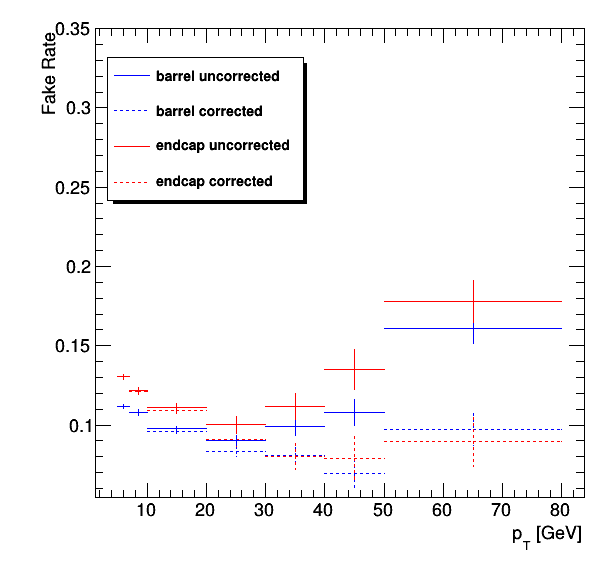
\includegraphics{Figures/RedBkg/FR/FR_SS_muons_2016.png}}}
    \subfigure [] {\resizebox{5.1cm}{!}{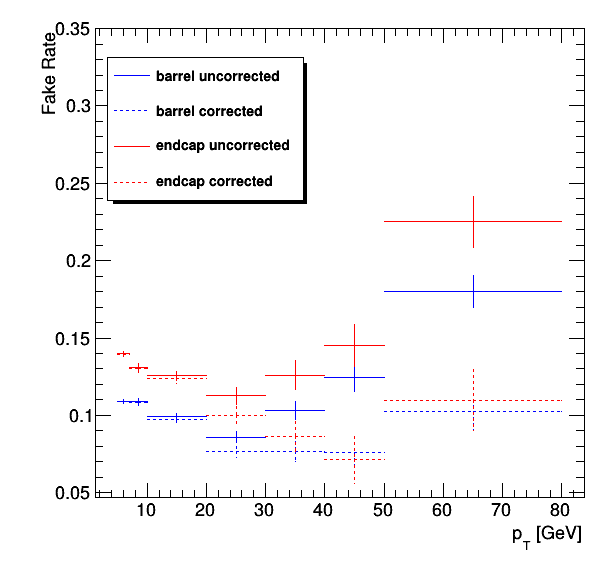
\includegraphics{Figures/RedBkg/FR/FR_SS_muons_2017.png}}}
    \subfigure [] {\resizebox{5.1cm}{!}{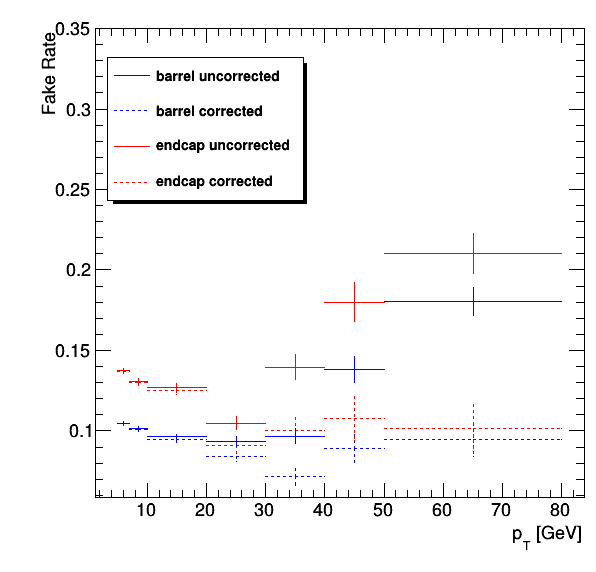
\includegraphics{Figures/RedBkg/FR/FR_SS_muons_2018.png}}}
\caption{Fake rates as a function of the probe $p_T$ for muons which satisfy the loose selection criteria, measured in
a $Z(\ell\ell)+\ell$ sample in the 2016 (top), 2017 (middle) and 2018 (bottom) data at $13$~TeV.
The barrel selection includes electrons (muons) up to $|\eta|$ = 1.479 (1.2). The fake rates are shown before (dotted lines) and after (plain line) the removal of the WZ contribution from the simulation.
}
\label{fig:fakerates}
\end{center}
\end{figure}
%=======  

For electrons, events where a radiated photon makes an asymmetric conversion, where one low $p_T$ leg is not identified, contribute to the $Z + e$ sample that is used to measure the electron fake rate. While the requirement $|M_{inv}(\ell_{1},\ell_{2}) - M_{Z}| < 7 $~GeV ("OS phase space") largely suppresses FSR of photons radiated off the lepton legs, these radiations occur at a much larger rate in the "SS phase space". 
As a result of this enhanced
contribution from conversions, the electron fake rates measured
within the SR phase space  are larger than the "OS fake rates".

However, the relative fraction of FSR conversions is not the same in the "SS phase space"
and in the control sample (defined below) where the fake rates will be applied. A correction
accounting for this difference must be applied to the fake rates measured within 
the SS phase space, in order to obtain
average fake rates that are appropriate for the control sample.
To determine this correction,
several fake rate samples of $Z(ll) + e$ events are defined by applying different 
cuts on $M_{inv}(\ell_{1},\ell_{2})$ or on $M_{inv}(\ell_{1},\ell_{2}, e)$.
In addition to the "OS fake rate sample", where $|M_{inv}(\ell_{1},\ell_{2}) - M_{Z}| < 7 $~GeV ensures
a minimal amount of conversions from FSR photons, one defines a sample that is
maximally enriched in FSR conversions by
$ | M_{inv}(\ell_{1},\ell_{2}, e) - M_Z | < $~5~GeV,
as well as samples with 
an intermediate contamination from FSR conversions (60~GeV $< M_{inv}(\ell_{1},\ell_{2}) < $ 120~GeV).
In each sample, one determines in several $(p_T, \eta)$ bins for the loose electron:
\begin{itemize}
 \item the fake rate ratio;
 \item the average value of the expected inner missing hits ($N_{miss. hits}$ in the following), variable useful to tag conversions. 
\end{itemize}
%

In a given $(p_T, \eta)$  bin, both the measured fake rate and the
average $ < N_{miss. hits} > $ are expected to grow linearly with the fraction
of conversions. 
Hence, one expects a linear dependence of the fake rate with respect to $ < N_{miss. hits} > $.
This linear behaviour is demonstrated in Figure~\ref{fig:FRvsNHits}, and linear fits are made
in each $(p_T, \eta)$  bin, which relate the fake rate to $ < N_{miss. hits} > $.
Finally, one looks at the loose electrons in the control sample where the fake rate will be applied, 
and $<N_{miss. hits}>$ is measured in each $(p_T, \eta)$ bin.
The proper average fake rate corresponding to the control sample is then determined from the
linear relation derived previously.
Figure~\ref{fig:FRAAcorrected} shows examples of the resulting corrected fake rates, together with the
fake rates measured in the SS phase space.
It can be seen that the correction for the actual fraction of conversions that is present in the
control sample lowers the fake rates considerably with respect to what is measured
in the SS phase space.
The determination of these corrected fake rates mostly suffers from the limited statistics of the
control sample, which translates into a large uncertainty on $<N_{miss. hits}>$, 
the error on each dot being the fake rate obtained from the linear relations using the error on the $<N_{miss. hits}>$.

\begin{figure}[!h]
\begin{center}
    \subfigure [] {\resizebox{7.75cm}{!}{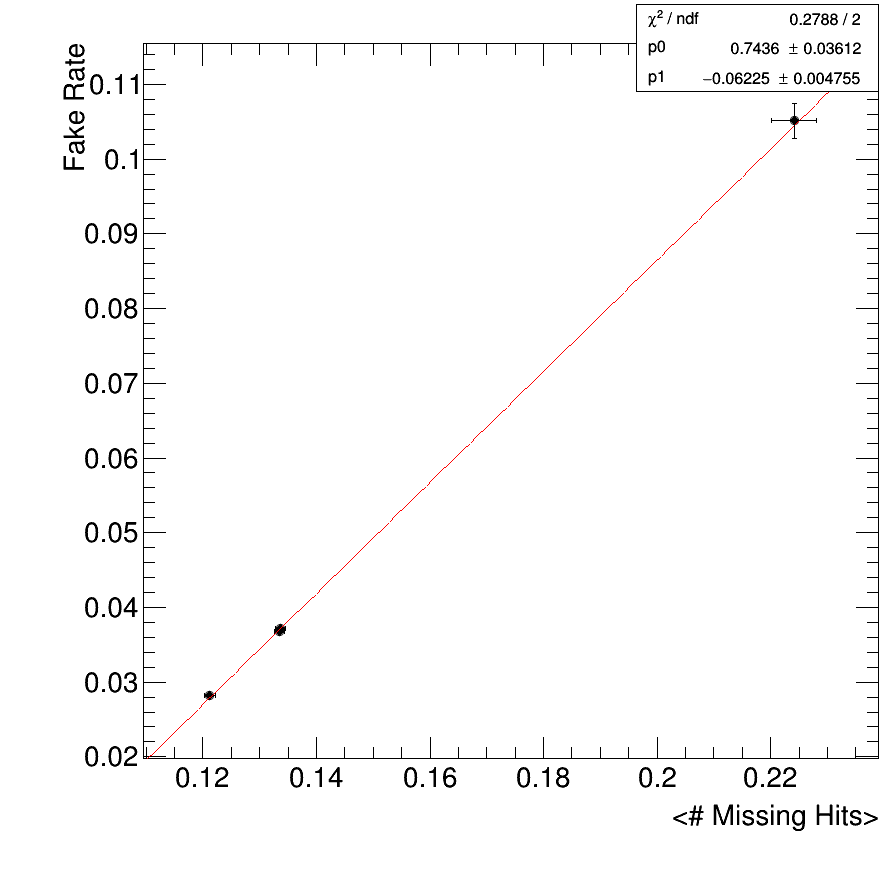
\includegraphics{Figures/RedBkg/FR_MissingHits_graph_eta_0_pT_0.png}}} 
    \subfigure [] {\resizebox{7.75cm}{!}{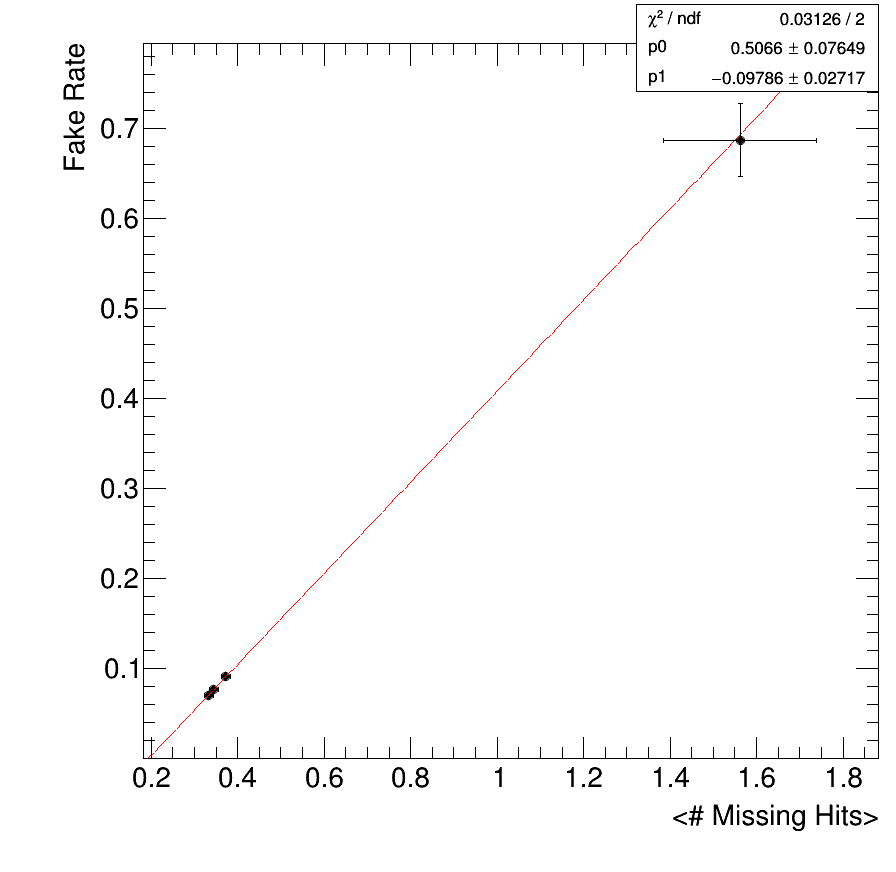
\includegraphics{Figures/RedBkg/FR_MissingHits_graph_eta_1_pT_4.png}}} 
\caption{
Examples of the correlation between the fake rate and the fraction of loose electrons 
for which the track has one missing hit in the pixel detector for  $7<p_T<10$~GeV electrons in the barrel (left) and for $30<p_T<40$~GeV electrons in the endcaps (right).
Each dot shows the measurements made in a given $Z$ + loose $e$ sample.
Results are produced at 13~TeV with 35.9~fb$^{-1}$ data.
}
\label{fig:FRvsNHits}
\end{center}
\end{figure}

%=======  
\begin{figure}[!htb]
\begin{center}
    \subfigure [] {\resizebox{5.1cm}{!}{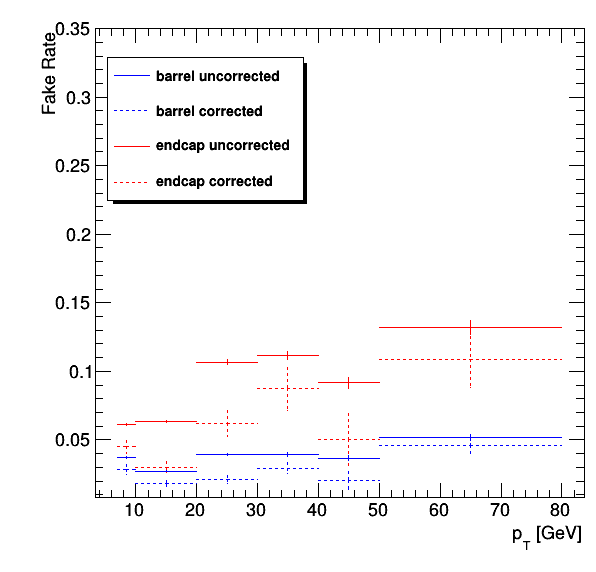
\includegraphics{Figures/RedBkg/FR/FR_SS_electrons_2016.png}}}
    \subfigure [] {\resizebox{5.1cm}{!}{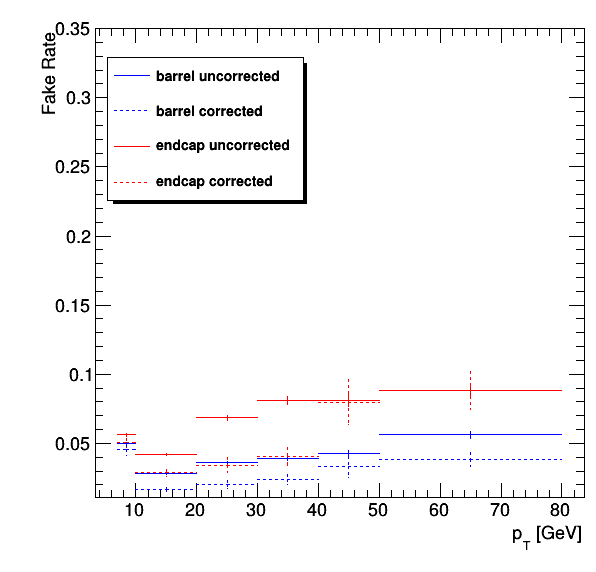
\includegraphics{Figures/RedBkg/FR/FR_SS_electrons_2017.png}}}
    \subfigure [] {\resizebox{5.1cm}{!}{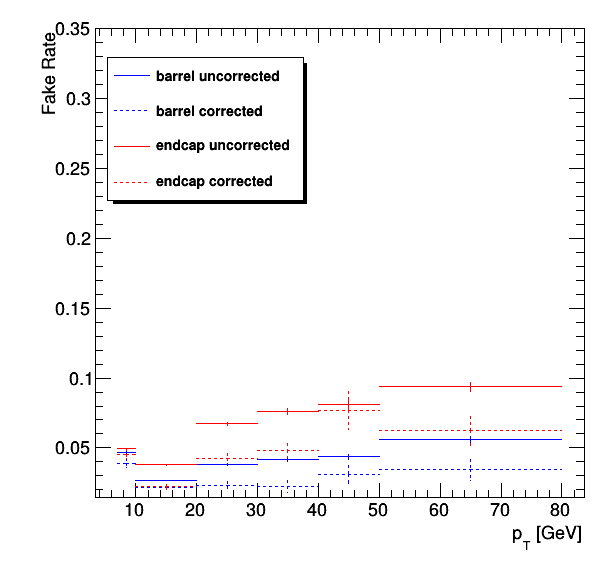
\includegraphics{Figures/RedBkg/FR/FR_SS_electrons_2018.png}}}
\caption{Average fake rates to be applied to the control sample of SS method (plain line), compared to
  the fake rates measured in the SS phase space (dotted line), for electrons in the barrel (blue) and in the endcaps (red).
  Results are produced at 13~TeV with 2016, 2017, and 2018 data.
}
\label{fig:FRAAcorrected}
\end{center}
\end{figure}
%=======  

% ============================================================================================================
%  FAKE RATE APPLICATION
% ============================================================================================================
\paragraph{Fake Rate Application (SS method)}
Figure~\ref{fig:ZjetControlRegionShapes13TeV} shows the invariant mass
distribution of events in control samples with SS-SF loose leptons,
for channels with loose electrons ($4e$ and $2\mu2e$) and channels
with loose muons ($4\mu$ and $2e2\mu$), for the 2018 dataset at $13$~TeV. 
The prediction from the Monte Carlo simulation is also shown.

A good agreement is achieved between data and MC for the channels
with loose electrons. The agreement is not as good for loose muons
but this has no impact on the final result as only data are used in the end.  

The differences in rates between OS and SS samples are estimated using data and are used to compute 
the correction factor in Eq.~\ref{eq:FakeRateAA} for the final data-driven estimation. 
They are given for each year in Table~\ref{tab:OSSS}.

\begin{table}[!htb]
% \scriptsize
\begin{center}
    \begin{tabular}{ | l | c | c | c |  c | }  \hline
   Channel  &  4e               &  2$\mu$2e          &  4$\mu$           &  2e2$\mu$        \\ \hline \hline   
   2016     &  1.00 $\pm$ 0.01  &  1.00 $\pm$ 0.01   &  1.00 $\pm$ 0.03  &  1.00 $\pm$ 0.03 \\ 
   2017     &  1.01 $\pm$ 0.01  &  1.00 $\pm$ 0.01   &  1.04 $\pm$ 0.03  &  1.01 $\pm$ 0.03 \\ 
   2018     &  1.01 $\pm$ 0.01  &  1.00 $\pm$ 0.01   &  1.03 $\pm$ 0.02  &  1.03 $\pm$ 0.02 \\ \hline
    \end{tabular}
    \caption{ The OS/SS ratios used to estimate the number of ZX events with the SS method for each final state in all three years. }
    \label{tab:OSSS}
\end{center}
\end{table}

%=======  
\begin{figure}[!h]
\begin{center}
\subfigure[]{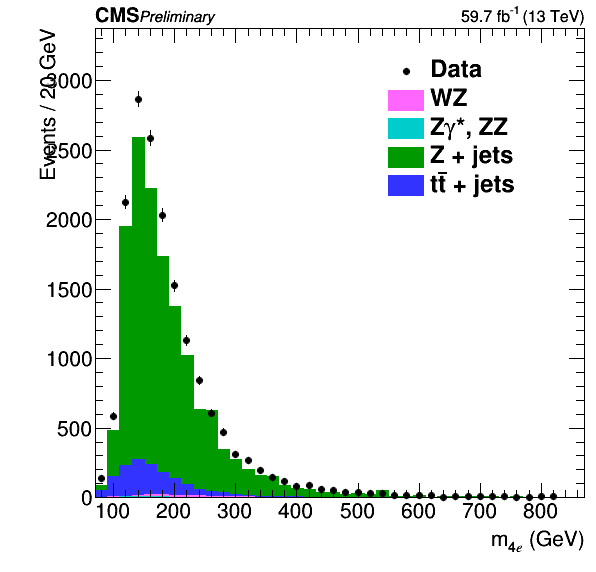
\includegraphics[width=0.45\textwidth]{Figures/RedBkg/M4l_dataMC/M4l_SS_4e_2018_Inclusive.png}} 
\subfigure[]{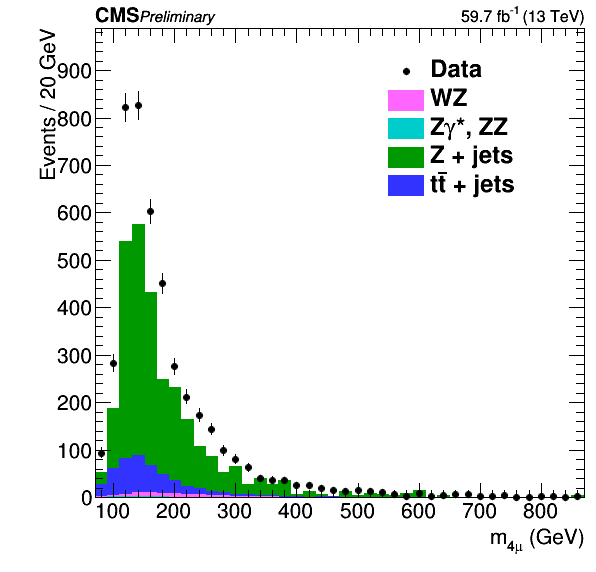
\includegraphics[width=0.45\textwidth]{Figures/RedBkg/M4l_dataMC/M4l_SS_4mu_2018_Inclusive.png}}  \\ 
\subfigure[]{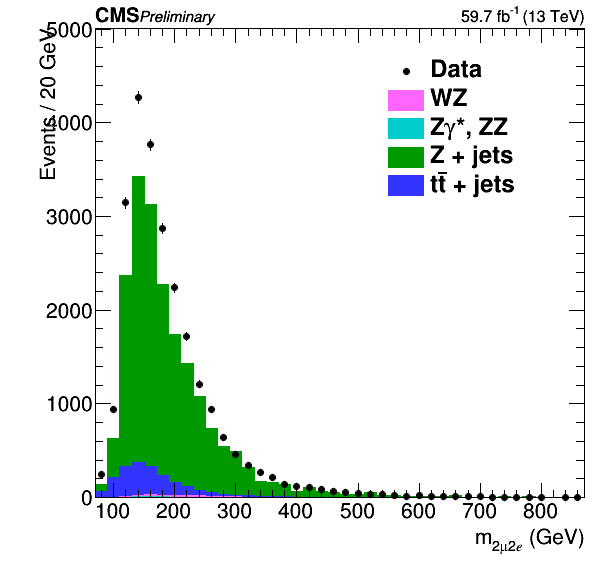
\includegraphics[width=0.45\textwidth]{Figures/RedBkg/M4l_dataMC/M4l_SS_2mu2e_2018_Inclusive.png}}  
\subfigure[]{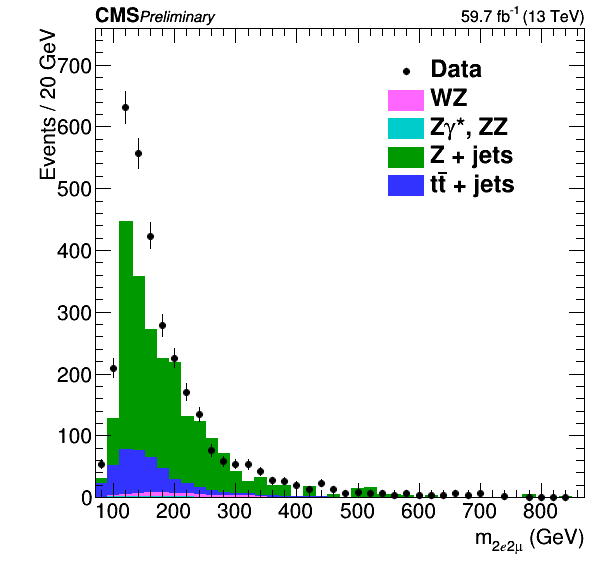
\includegraphics[width=0.45\textwidth]{Figures/RedBkg/M4l_dataMC/M4l_SS_2e2mu_2018_Inclusive.png}} \\ 
\caption{Invariant mass distribution of the events selected in the SS-SF control samples for all the considered final states in 2018 data:
$4e$ (a), $4\mu$ (b), $2\mu2e$ (c) and $2e2\mu$ (d).  
\label{fig:ZjetControlRegionShapes13TeV}}
\end{center}
\end{figure}
%=======  

The event yields expected from the Z+X in the signal region, in the mass range  $m_{4 \ell} > 70~\GeVcc$, are calculated for each final state.
%and for each of the 22 STXS Stage 1.1 categories defined in Section~\ref{sec:categorization}. An example for the $4e$ final state in 2018 data is shown in Table~\ref{tab:ZjetResultsAA_4e}.
%The statistical error is due to the event statistics in the control region, while the systematic one is due to error introduced with the missing hits based correction for electrons and the uncertanty in the fake rates in the muon case. 
The background is due to the systematic introduced when estimating the background composition. 
The total error is obtained with a quadrature sum for the statistical, background composition and correction systematics. 
Table~\ref{tab:SSyields} shows the expected number of events in the signal regions 
from the reducible background processes at $13$~TeV for each considered final state 
and for all three years using the SS method.
%
%
%\begin{table}[htb!]
%\begin{center}
%\small
%\begin{tabular}{ l | c | c | c | c | c | c}
%\hline
%\hline
%Category & exp. $N^{\rm Z+X}$ in SR & (stat.) & (syst. - FR) & (syst - Bkg comp) & Total unc.\\
%\hline
%\hline
%ggH\_0J\_PTH\_0\_10        & 0.35 & $\pm 0.02$ & $\pm 0.07 $    & $\pm 0.11 $  & $\pm 0.13 $ \\
%\hline
%ggH\_0J\_PTH\_10\_200      & 6.75 & $\pm 0.08$ & $\pm 1.40 $    & $\pm 2.03 $  & $\pm 2.48 $ \\
%\hline
%ggH\_1J\_PTH\_0\_60        & 2.18 & $\pm 0.04$ & $\pm 0.44 $    & $\pm 0.65 $  & $\pm 0.79 $ \\
%\hline
%ggH\_1J\_PTH\_60\_120      & 1.51 & $\pm 0.04$ & $\pm 0.32 $    & $\pm 0.45 $  & $\pm 0.56 $ \\
%\hline
%ggH\_1J\_PTH\_120\_200     & 0.53 & $\pm 0.02$ & $\pm 0.12 $    & $\pm 0.16 $  & $\pm 0.20 $ \\
%\hline
%ggH\_2J\_PTH\_0\_60        & 0.65 & $\pm 0.02$ & $\pm 0.13 $    & $\pm 0.20 $  & $\pm 0.23 $ \\
%\hline
%ggH\_2J\_PTH\_60\_120      & 0.74 & $\pm 0.03$ & $\pm 0.16 $    & $\pm 0.22 $  & $\pm 0.27 $ \\
%\hline
%ggH\_2J\_PTH\_120\_200     & 0.31 & $\pm 0.02$ & $\pm 0.07 $    & $\pm 0.09 $  & $\pm 0.12 $ \\
%\hline
%ggH\_PTH\_200              & 0.45 & $\pm 0.02$ & $\pm 0.11 $    & $\pm 0.14 $  & $\pm 0.17 $ \\
%\hline
%ggH\_VBF                   & 0.28 & $\pm 0.02$ & $\pm 0.06 $    & $\pm 0.08 $  & $\pm 0.10 $ \\
%\hline
%VBF\_1j                    & 0.47 & $\pm 0.02$ & $\pm 0.09 $    & $\pm 0.14 $  & $\pm 0.17 $ \\
%\hline
%VBF\_2j                    & 0.30 & $\pm 0.02$ & $\pm 0.06 $    & $\pm 0.09 $  & $\pm 0.11 $ \\
%\hline
%VBF\_2j\_mjj\_350\_700\_2j & 0.02 & $\pm 0.00$ & $\pm 0.00 $    & $\pm 0.01 $  & $\pm 0.01 $ \\
%\hline
%VBF\_2j\_mjj\_GT700\_2j    & 0.02 & $\pm 0.002$ & $\pm 0.003 $  & $\pm 0.01 $  & $\pm 0.01 $ \\
%\hline
%VBF\_2j\_mjj\_GT350\_3j    & 0.40 & $\pm 0.02$ & $\pm 0.09 $    & $\pm 0.12 $  & $\pm 0.15 $ \\
%\hline
%VBF\_GT200\_2J             & 0.03 & $\pm 0.01$ & $\pm 0.01 $    & $\pm 0.01 $  & $\pm 0.01 $ \\
%\hline
%VH\_Had                    & 0.57 & $\pm 0.02$ & $\pm 0.12 $    & $\pm 0.17 $  & $\pm 0.21 $ \\
%\hline
%VBF\_rest\_VH              & 0.10 & $\pm 0.01$ & $\pm 0.02 $    & $\pm 0.03 $  & $\pm 0.04 $ \\
%\hline
%VH\_lep\_0\_150            & 0.13 & $\pm 0.01$ & $\pm 0.03 $    & $\pm 0.04 $  & $\pm 0.05 $ \\
%\hline
%VH\_Lep\_GT150             & 0.01 & $\pm 0.00$ & $\pm 0.00 $    & $\pm 0.00 $  & $\pm 0.00 $ \\
%\hline
%ttH\_Lep                   & 0.04 & $\pm 0.01$ & $\pm 0.01 $    & $\pm 0.01 $  & $\pm 0.02 $ \\
%\hline
%ttH\_Had                   & 0.19 & $\pm 0.01$ & $\pm 0.04 $    & $\pm 0.06 $  & $\pm 0.07 $ \\
%\hline
%\hline
%Inclusive                  & 16.0 & $\pm 0.12$ & $\pm 3.34 $    & $\pm 4.8 $ & $\pm 5.85 $ \\
%\hline
%\hline
%\end{tabular}
%\end{center}
%\caption{Number of $4e$ events in the SS-SF control region for 59.7~fb$^{-1}$ of 2018 data, and expected number of Z+X$\to4\Pe$ events in the signal region as predicted from the SS method. The total uncertainty associated to the SS measurement is shown in the table together with the splitting in its three contributions: statistical error and both systematic errors due to fake rate variation and background composition.
%\label{tab:ZjetResultsAA_4e}}
%\end{table}
%

\begin{table}[!htb]
\begin{center}
     \begin{tabular}{| l | c | c | c | c |} \hline
Channel & 4e               & 4$\mu$          & 2e2$\mu$        & 2$\mu$2e        \\ \hline \hline
2016    & $ 13.0 \pm 5.4 $ & $29.7 \pm 9.1$  & $24.8 \pm 7.6$  & $16.7 \pm 7.0$  \\
2017    & $ 10.9 \pm 4.0 $ & $33.6 \pm 10.3$ & $26.3 \pm 8.1$  & $14.7 \pm 5.5$  \\
2018    & $ 16.0 \pm 5.9 $ & $52.2 \pm 15.8$ & $37.4 \pm 11.4$ & $23.3 \pm 8.5$  \\ \hline
        \end{tabular}
\end{center}
    \caption{ The contribution of reducible background
    processes in the signal region predicted from measurements in 2016, 2017 and 2018 data
    using the SS method. The predictions correspond to 35.9, 41.5 and 59.7~fb$^{-1}$ of data at $13$~TeV, respectively.}
     \label{tab:SSyields}
\end{table}

\paragraph{Fake Rate in the VBF-tagged categories}
The FR are currently evaluated inclusively in the analysis: in fact, an average fake rate is used to evaluate ZX yields in each STXS category instead of dedicated ones.
Given that the VBF category can be particularly affected by this approach, a detailed study of the FR variation in different Z+L phase spaces designed to mimic VBF has been performed using 2018 data. 
However, a realistic design of the VBF phase space is not completely reproducible in the three leptons CR without exploiting the information given by the kinematic discriminants.
In order to identify events targeting VBF-tagged categories, the following requirements on jets are applied:
\begin{itemize} 
\item an angular separation between the additional lepton and each jet larger than 0.4, otherwise the jet is discarded;       
\item the presence of two or three jets and at most one b tagged jet OR at least four jets without b tagged jets;
\item an angular separation between the pair of two leading jets larger than 0.5 and a dijet invariant mass greater than 450 GeV. 
\end{itemize}

Futhermore, FR in the CR Z+L with 0/1/2 jets have been studied as well as the FR in the phase space complementary to the VBF-like one.
Figure~\ref{fig:FRSSperCat} shows the FR curves obtained in each category for both electrons and muons in the barrel and endcap region using the SS method and Figure~\ref{fig:FROSperCat} shows the same distributions using the OS method. 
While the curve in the "non VBF-tagged'' region is perfectly in agreement with the inclusive one (as a result of the contribution of the 0/1/2 jet categories),   
the FR variation in the 0/1/2 jets and VBF-like categories is significant, especially for muons.
As a consequence, large discrepancies are observed in the final estimated yields in VBF categories (Table~\ref{tab:VBFyields}).

%=======  
\begin{figure}[!h]
\begin{center}
\subfigure[]{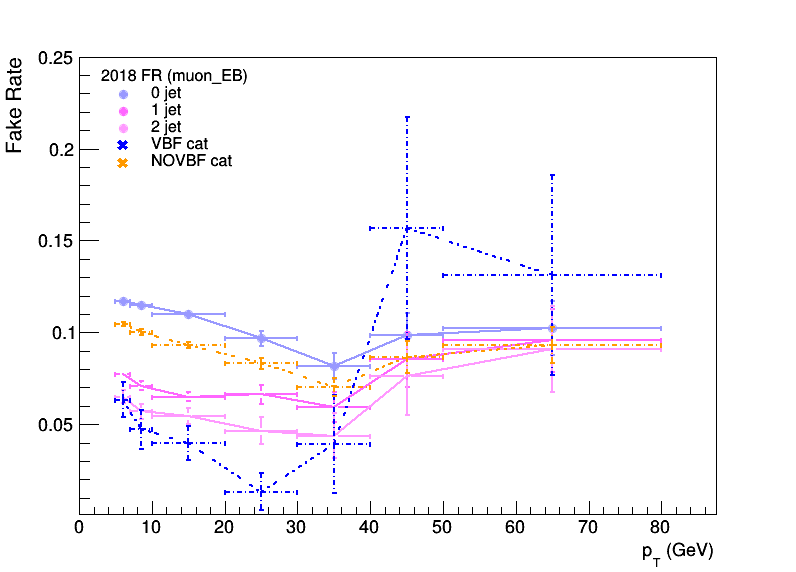
\includegraphics[width=0.45\textwidth]{Figures/RedBkg/FR/allCat_FR_muon_EB_2018_SS.png}} 
\subfigure[]{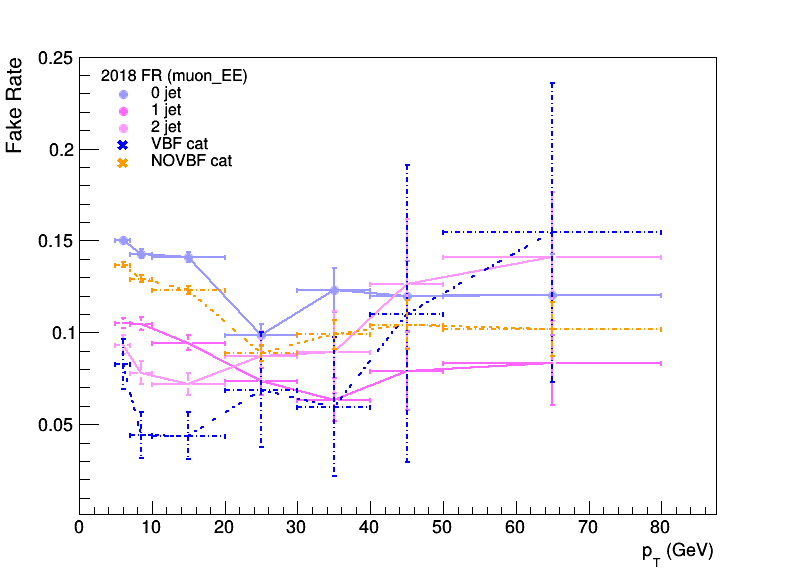
\includegraphics[width=0.45\textwidth]{Figures/RedBkg/FR/allCat_FR_muon_EE_2018_SS.png}}}  \\ 
\subfigure[]{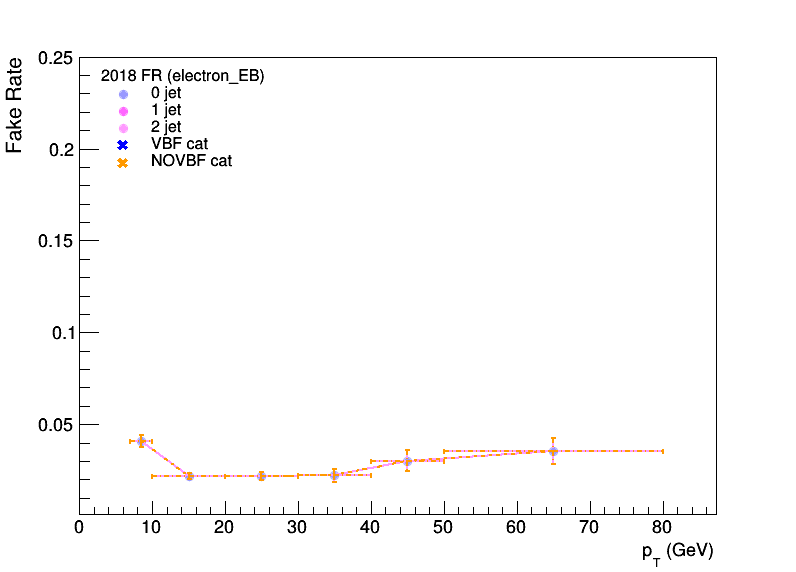
\includegraphics[width=0.45\textwidth]{Figures/RedBkg/FR/allCat_FR_electron_EB_2018_SS.png}}}  
\subfigure[]{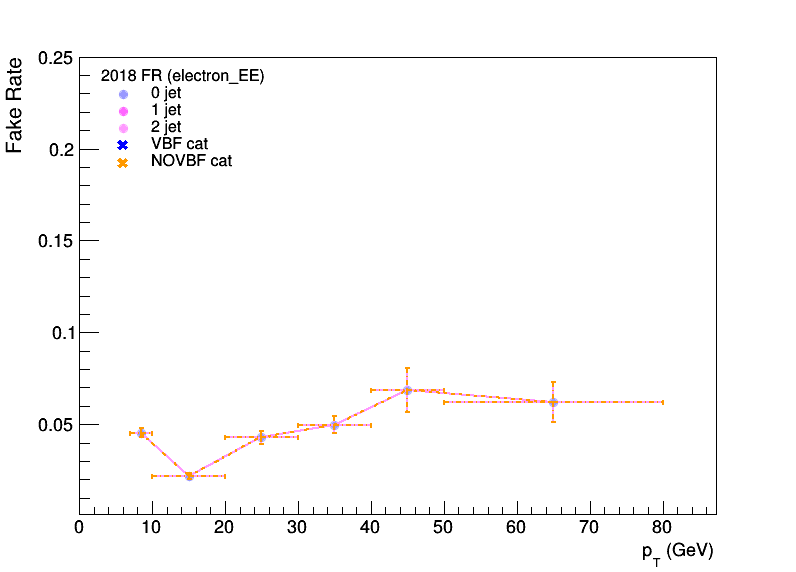
\includegraphics[width=0.45\textwidth]{Figures/RedBkg/FR/allCat_FR_electron_EE_2018_SS.png}}} \\ 
\caption{FR curves in the 0/1/2/VBF-tagged and non VBF-tagged categories for muons (top) and electrons (bottom) in the barrel (left) and endcap (right) region obtained using SS method.   
\label{fig:FRSSperCat}}
\end{center}
\end{figure}
%=======    
\begin{figure}[!h]
\begin{center}
\subfigure[]{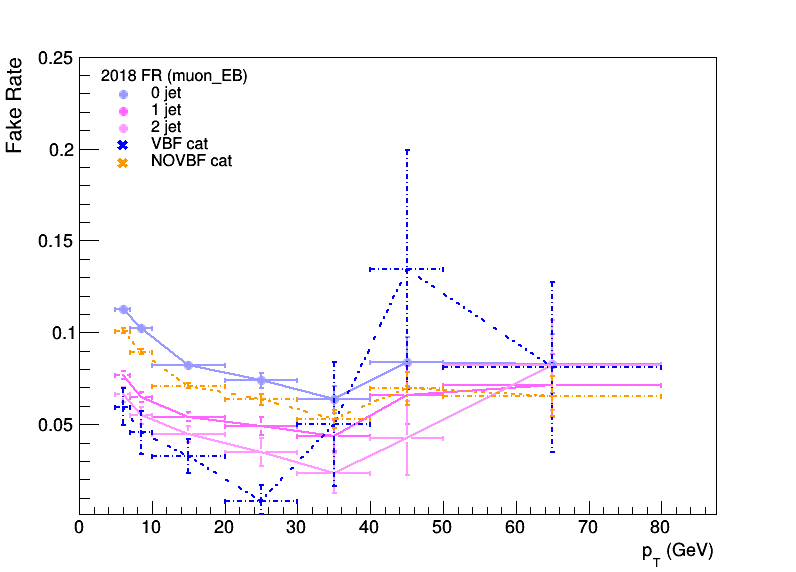
\includegraphics[width=0.45\textwidth]{Figures/RedBkg/FR/allCat_FR_muon_EB_2018_OS.png}} 
\subfigure[]{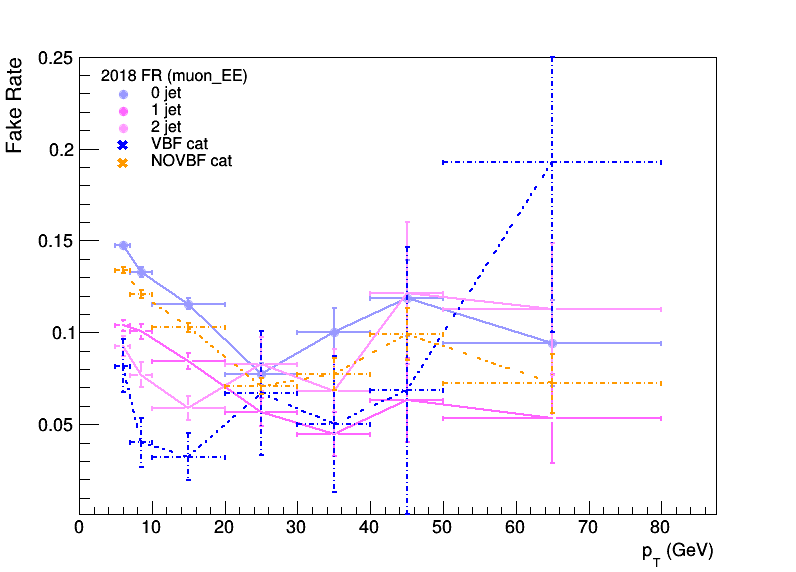
\includegraphics[width=0.45\textwidth]{Figures/RedBkg/FR/allCat_FR_muon_EE_2018_OS.png}}}  \\ 
\subfigure[]{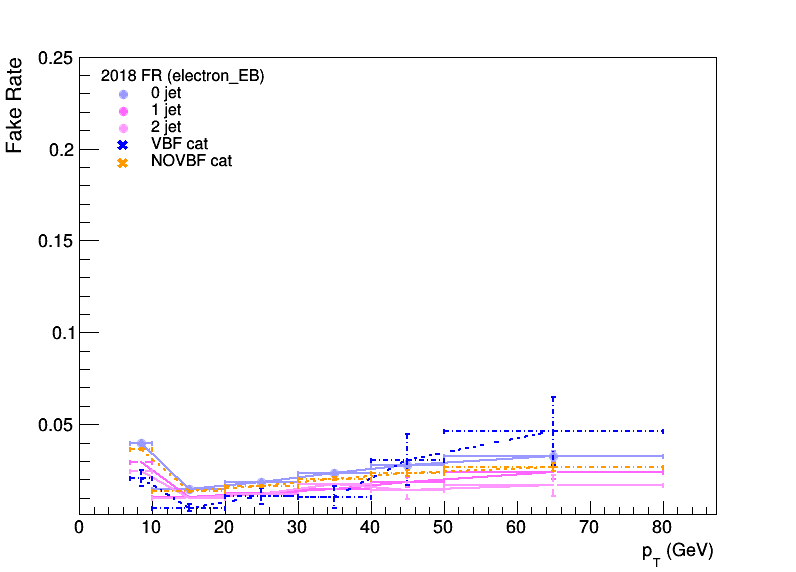
\includegraphics[width=0.45\textwidth]{Figures/RedBkg/FR/allCat_FR_electron_EB_2018_OS.png}}}  
\subfigure[]{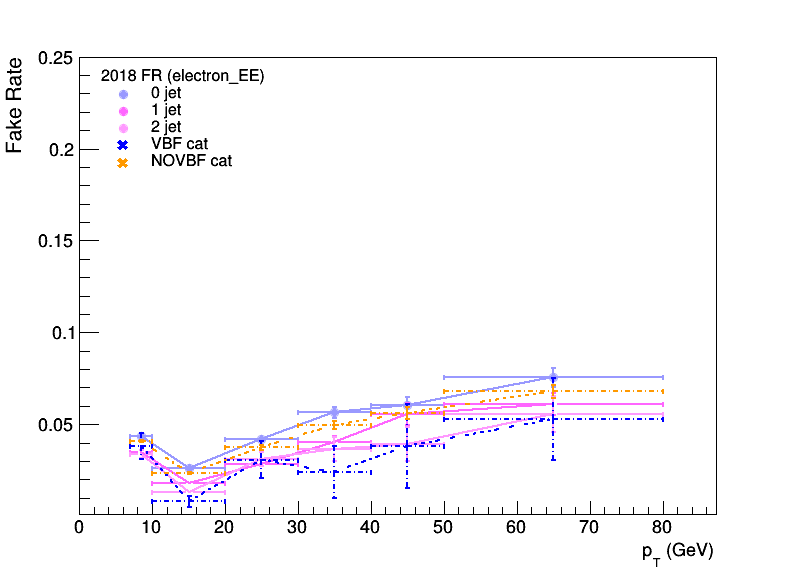
\includegraphics[width=0.45\textwidth]{Figures/RedBkg/FR/allCat_FR_electron_EE_2018_OS.png}}} \\ 
\caption{FR curves in the 0/1/2/VBF-tagged and non VBF-tagged categories for muons (top) and electrons (bottom) in the barrel (left) and endcap (right) region obtained using OS method.   
\label{fig:FRSSperCat}}
\end{center}
\end{figure}
%=======  

\begin{table}[!h]
        \begin{center}
                \caption{
                Comparison between combined ZX yields in the VBF-tagged categories using inclusive and dedicated FR. 
                \label{tab:VBFyields}
                        }
    \renewcommand{\arraystretch}{1.5}
    \begin{tabular}{c|cccc|cccc}
        & \multicolumn{4}{c|}{Inclusive FR} & \multicolumn{4}{c}{Dedicated FR} \\
        CATEGORY                   & $4l$  & $4\mu$ & $4e$ & $2e2\mu$  & $4l$ & $4\mu$ & $4e$ & $2e2\mu$ \\
        \hline
        VBF\_1j                     & 1.047 & 0.391 & 0.147 & 0.509    & 0.663 & 0.185 & 0.113 & 0.365  \\
        VBF\_2j                     & 0.882 & 0.295 & 0.097 & 0.490    & 0.054 & 0.011 & 0.016 & 0.028  \\
        VBF\_2j\_mjj\_350\_700\_2j  & 0.040 & 0.026 & 0.003 & 0.011    & 0.004 & 0.000 & 0.000 & 0.004  \\
        VBF\_2j\_mjj\_GT700\_2j     & 0.016 & 0.013 & 0.002 & 0.001    & 0.091 & 0.018 & 0.039 & 0.034  \\
        VBF\_2j\_mjj\_GT350\_3j     & 0.997 & 0.444 & 0.104 & 0.450    & 0.001 & 0.001 & 0.000 & 0.000  \\
        VBF\_GT200\_2J              & 0.021 & 0.019 & 0.001 & 0.001    & 0.015 & 0.001 & 0.001 & 0.014  \\
        \hline                      
        Inclusive VBF               & 3.002 & 1.188 & 0.353 & 1.461    & 0.828 & 0.216 & 0.169 & 0.444  \\
        \hline


\end{tabular}
        \end{center}
\end{table}

In principle, the uncertainty on the background composition of the CR was designed to cover for this effect, but considering that the effect seems very large, 
the possible impact on the analysis has been checked explicitely. 
An extreme situation has been studied by inflating the Z+X uncertainty by 100$\%$ in the datacards in VBF-tagged categories and comparing stage 0 signal strengths, 
both expected and observed, using the standard Z+X uncertainty and inflating it in VBF categories (Table~\ref{tab:inflatedMu}). 
The results show that the expected uncertainty does not change and the observed signal strengths change only very slightly (2nd digit) within the uncertainties. 

\begin{table}[!h]
        \begin{center}
                \caption{
                Comparison between the best-fit values and $\pm 1\sigma$ uncertainties for the expected and observed signal-strength modifiers,
                inflating ZX uncertainties in VBF categories by 100$\%$ and keeping nominal ZX uncertainties.
                \label{tab:inflatedMu}
                        }
    \renewcommand{\arraystretch}{1.5}
    \begin{tabular}{c|cc|cc}
        & \multicolumn{2}{c|}{Inflated ZX uncertainty} & \multicolumn{2}{c}{Nominal ZX uncertainty} \\
        & Expected  & Observed & Expected & Observed \\
        \hline
        $\mu_{\ttH,\tH}$       & $1.00~^{+1.36}_{-0.78}~$ & $0.23 ^{+0.95}_{-0.23}$   & $1.00~^{+1.36}_{-0.78}~$ & $0.22 ^{+0.95}_{-0.22}$ \\
        $\mu_{\WH}$            & $1.00~^{+2.01}_{-1.00}~$ & $1.68 ^{+1.76}_{-1.44}$   & $1.00~^{+2.01}_{-1.00}~$ & $1.71 ^{+1.79}_{-1.71}$ \\
        $\mu_{\ZH}$            & $1.00~^{+8.33}_{-1.00}~$ & $0.00 ^{+5.24}_{-0.00}$   & $1.00~^{+8.33}_{-1.00}~$ & $0.00 ^{+5.44}_{-0.00}$ \\
        $\mu_{\mathrm{VBF}}$   & $1.00~^{+0.56}_{-0.46}~$ & $0.54 ^{+0.51}_{-0.41}$   & $1.00~^{+0.56}_{-0.46}~$ & $0.56 ^{+0.50}_{-0.41}$ \\
        $\mu_{\Pg\Pg\PH,\bbH}$ & $1.00~^{+0.16}_{-0.14}~$ & $1.02 ^{+0.15}_{-0.13}$   & $1.00~^{+0.16}_{-0.14}~$ & $1.03 ^{+0.15}_{-0.13}$ \\
        \hline
\end{tabular}
        \end{center}
\end{table}



In conclusion, the current approach based on an inclusive FR assumed identical for all the production categories is not correct because FR is indeed different for VBF-tagged categories. 
Nevertheless, the final impact on the analysis is found to be not significant due to the kinematic discriminant used in the fit and the fact that Z+X yields
are rather insignificant, so that the current strategy is kept for this analysis and more effort to have a category specific Z+X estimate in the future Run 3 analysis will be invested.
